\section*{08/07/2022 --- Estabilidade local e global}
\markboth{Estabilidade local e global}{08/07/2022}
\noindent\textbf{\sffamily Exercício 1.}
	Encontre $H$ de Lyapunov que comprove a estabilidade do sistema descrito por 
	%
	\[
		\dddot{x} = -6\ddot{x} -12\dot{x} -8x.
	\]
	%

\noindent\textbf{\sffamily Exercício 2.}
	Mostre que a equação de Van der Pol,
	%
	\[
		\ddot{x} = -kx - \alpha(1-x^2)\dot{x},
		\quad k, \alpha>0,
	\]
	%
	é estável para $x$ suficientemente pequeno. \\
	%

\noindent\textbf{\sffamily Exercício 3.}
	Analise a estabilidade de Lyapunov do pêndulo com antrito,
	%
	\[
		\ddot{x} = -\sin x -\alpha \dot{x}, \quad\alpha>0.
	\]
	%	

\noindent\textbf{\sffamily Exercício 4.}
	Analise a estabilidade do sistema descrito por
	%
	\[
		\ddot{\theta} = -2\theta -4\dot{\theta} + \theta^3.
	\]
	%	

\noindent\rule{\textwidth}{0.5pt}
\noindent
\textbf{\sffamily Exercício 1 --- solução.} \\
	Existe uma forma geral para encontrar funções/estabilidade de Lyapunov quando o sistema é linear. 
	Ela consiste em determinar matriz $P>0$ simétrica tal que $H(X) = X^TPX$ é de Lyapunov. 
	Visto que $\dot{X} = AX$, esse último requerimento se traduz em 
	%
	\begin{align*}
		0 >
		\dot{H} &= \dot{X}^TPX + X^TP\dot{X} \\
		        &= (AX)^TPX + X^TP(AX) \\
		        &= X^TA^TPX + X^TPAX \\
		        &= X^T(A^TP + PA)X 
		\iff
		A^TP + PA < 0.
	\end{align*}
	%
	Neste exercício, vamos impor $A^TP + PA = -\I$.
	Podemos encontrar tal $P$ simplesmente rodando o comando {\tt P = lyap(A', I)} no Matlab, conforme o código abaixo. 
	%
	\lstinputlisting[%
		language=Matlab, 
		caption=Código Matlab para encontrar $H$ de Lyapunov
	]{lyapunovLinear.m}
	%
	No código, assumi que 
	$x_1 := x$, 
	$x_2 := \dot{x}$, e
	$x_3 := \ddot{x}$ 
	formam o vetor de estados 
	$X = \begin{bmatrix} 
		 	x_1 & x_2 & x_3
	 	 \end{bmatrix}^T$.
 	Ao final, ficamos com		
	%
	\[
		P = 
	    \frac{1}{128}
	    \begin{pmatrix}
	    	224 &  392 & 8 \\
	    	392  & 2248 & 266 \\
	    	8    &  266 & 55
	    \end{pmatrix},	    
	\]
	%	
	e o sistema é (exponencialmente) estável, como esperado. \\

\noindent
\textbf{\sffamily Exercício 2 --- solução.} \\
	Tomando $H(x) = \frac{kx^2}{2} + \frac{\dot{x}}{2}$, temos 
	%
	\begin{align*}
		\dot{H} &= kx\dot{x} + \dot{x}\ddot{x} \\
		        &= \dot{x}(kx + \ddot{x}) \\
		        &= -\alpha\dot{x}^2(1-x^2) \\
		\implies \dot{H} &\leq 0 \iff |x|\leq 1.
	\end{align*}
	%
	Assim, por mais que $H$ seja positiva definida em $\R$, só podemos garantir estabilidade (assintótica) em $[-1, 1]$. \\

\noindent	
\textbf{\sffamily Exercício 3 --- solução.} \\
	Podemos tomar a energia do sistema como candidata à função de Lyapunov:
	%
	\begin{align*}
		H(x) = (1-\cos x) + \frac{\dot{x}^2}{2} \implies
		\dot{H} &= \dot{x}\sin x + \dot{x}\ddot{x} \\
		        &= \dot{x}(\sin x + \ddot{x}) \\
		        &= -\alpha\dot{x}^2. 
	\end{align*}
	%
	A rigor, embora a derivada seja não positiva em $\R$, a estabilidade segundo a $H$ tomada só é provada para $x\in(-\pi/2, \pi/2)$, conjunto onde a função é positiva definida. \\
	
\noindent
\textbf{\sffamily Exercício 4 --- solução.} \\
	Apenas do termo cúbico em $\theta$, o linearizado tangente da EDO nos diz que o sistema é estável em 
	$(\theta, \dot{\theta}) = (0,0)$. 
	Espera-se então que essa convergência seja apenas local; de fato, tomar 
	%
	\[
		H(\theta) = 2\frac{\theta^2}{2} + 
		            \frac{\dot{\theta}^2}{2} -
		            \frac{\theta^4}{4}
	\]
	%
	implica em
	%
	\begin{align*}
		\dot{H} &= 2\theta\dot{\theta} +
		           \dot{\theta}\ddot{\theta} -
		           \theta^3\dot{\theta} \\
		        &= \dot{\theta}(2\theta + \ddot{\theta} - \theta^3) \\
		        &= -4\dot{\theta}^2,
	\end{align*}
	%
	que é não positiva para todo $\theta\in\R$. 
	Entretanto, como $H$ não é necessariamente positivo definida, essa estabilidade é local. 
	O retrato de fase da EDO é de fato um tanto estranho (região $[-3,3]\times[-3,3]$).
	%
	\begin{figure}[H]\centering
		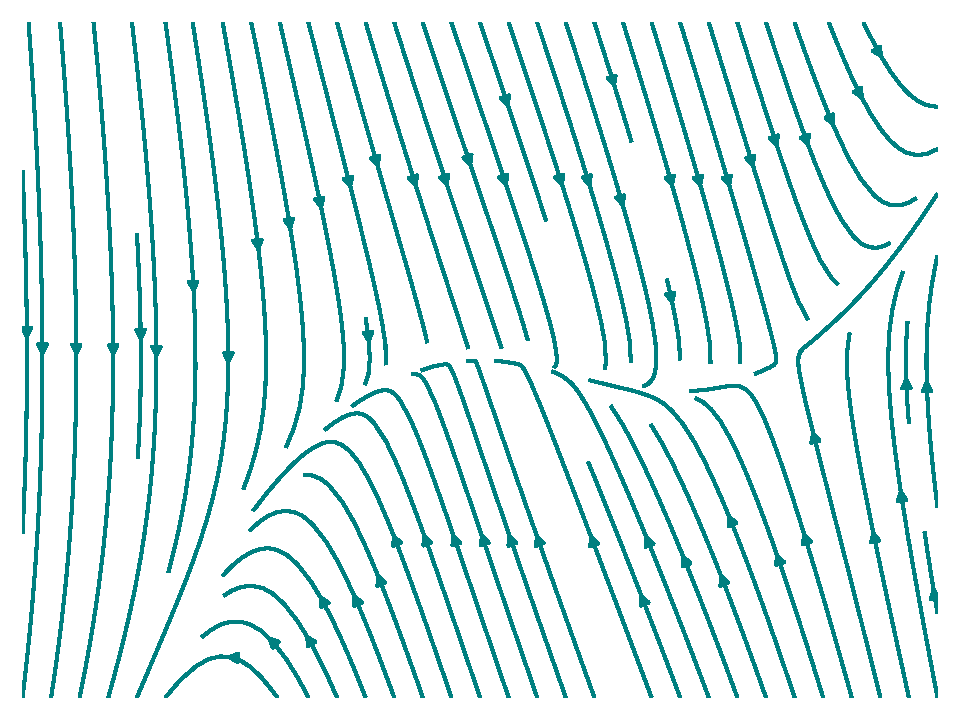
\includegraphics[width=7cm]{sistema com 2theta.pdf}
	\end{figure}
	%
























